%header
\documentclass{beamer}
\usepackage{beamerthemeshadow}
\usepackage[latin1]{inputenc}
\usepackage[english]{babel}
\usepackage{amsmath}
\usepackage{amssymb}
\usepackage{color}
\usepackage{lscape}
\usepackage{alltt}
\usepackage{array}
\usepackage{color}
\usepackage{listings}
\usepackage{graphicx}
\usepackage{csquotes}
\usepackage{caption}
\usepackage{subcaption}

\setbeamertemplate{footline}[frame number]
\graphicspath{ {images/} }

\begin{document}

% title page
\title{ Smart Habits Smart Savings}
\author{by Dorian Guzman and Nicolas Holland\\
\ \\
Freiburg Hackathon\\
\ \\
}


\frame{\titlepage} 

\frame{\frametitle{Energy Production Mix}
\begin{center}
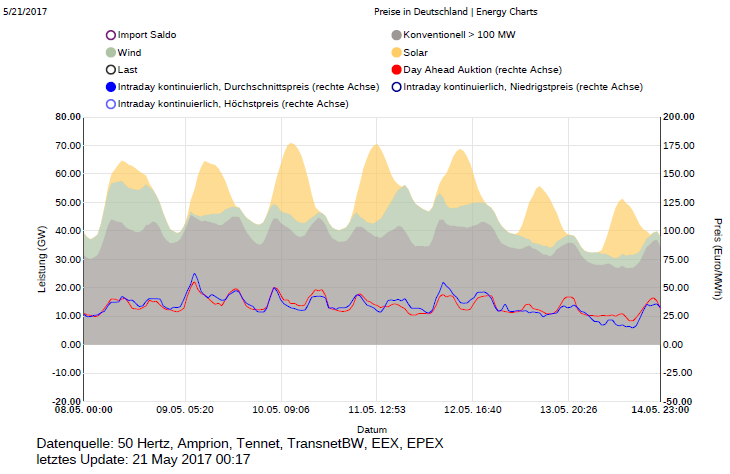
\includegraphics[scale=.55]{energy_charts}
\end{center}
}

\frame{\frametitle{Data Sources}

\begin{itemize}
\item DEBS 2014 Grand Challenge: Smart homes

\begin{itemize}
\item House id
\item Household id
\item Device id
\item Measurements per second
\end{itemize}

\item www.50hertz.com/en/Grid-Data
\begin{itemize}
\item Grid feed-in
\item Windpower
\item Photovoltaics
\item Measurements per 15 minutes
\end{itemize}

\end{itemize}

}

\frame{\frametitle{Crunching the Numbers}
\begin{center}
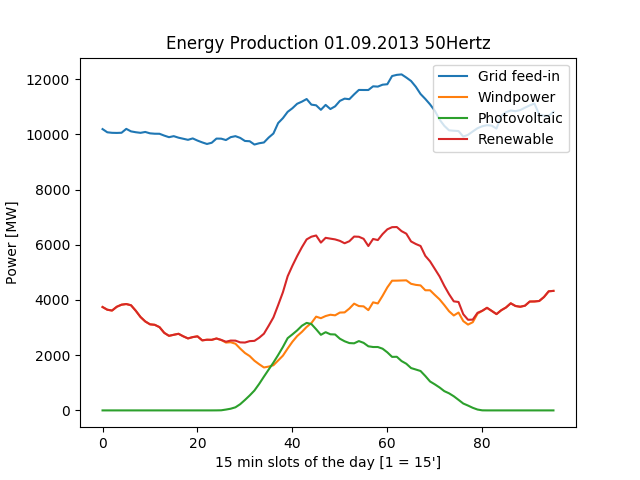
\includegraphics[scale=.55]{Production}
\end{center}
}

\frame{\frametitle{Crunching the Numbers}
\begin{center}
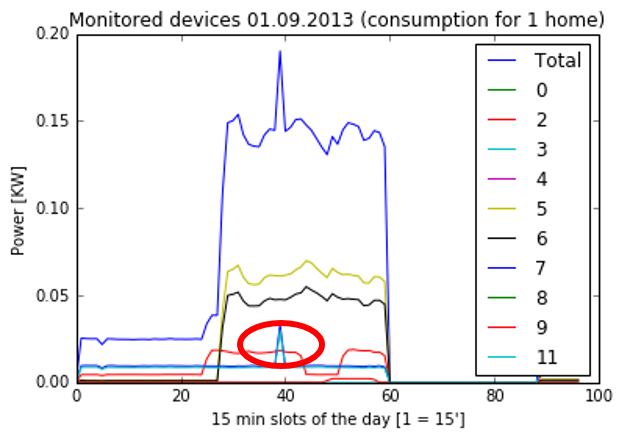
\includegraphics[scale=.8]{consumption_devices_circles}
\end{center}
}

\frame{\frametitle{Crunching the Numbers}
\begin{center}
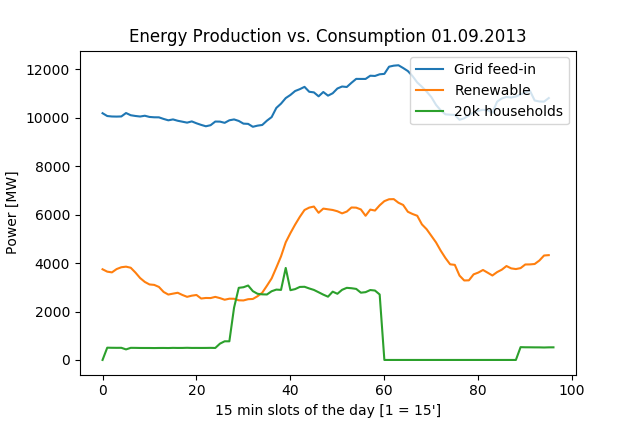
\includegraphics[scale=.55]{ProductionConsumtion}
\end{center}
}

\frame{\frametitle{Optimizing the Consumption Habit}
Let $R$ be renewable energy production, $C$ consumption habit, $T$ total consumption over one day, $D_i$ device consumption.
\ \\
\begin{minipage}{.5\textwidth}
Total Consumption:
\begin{align*}
\min_C \Vert R - C \Vert\\
\text{s.t.} \Vert C\Vert = T
\end{align*}
  \end{minipage}%
  \begin{minipage}{.5\textwidth}
    \centering
    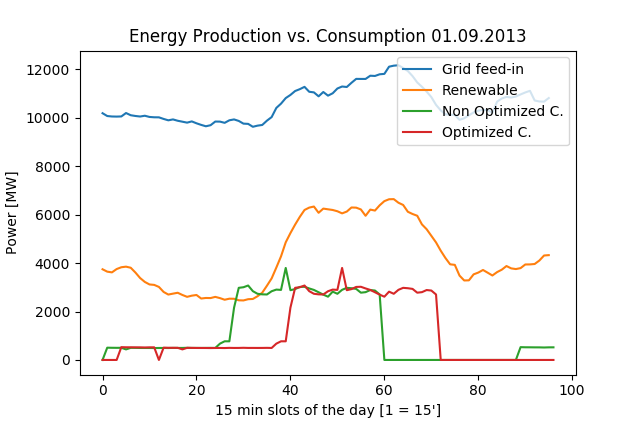
\includegraphics[scale=0.35]{SimpleOpt}
  \end{minipage}
  
\begin{minipage}{.5\textwidth}
Device Specific Consumption:
\begin{align*}
\min_{D_{i\in I}} \Vert R - D_i \Vert\\
\text{s.t.} \Vert \sum_i D_i\Vert = T
\end{align*}
  \end{minipage}%
  \begin{minipage}{.5\textwidth}
    \centering
    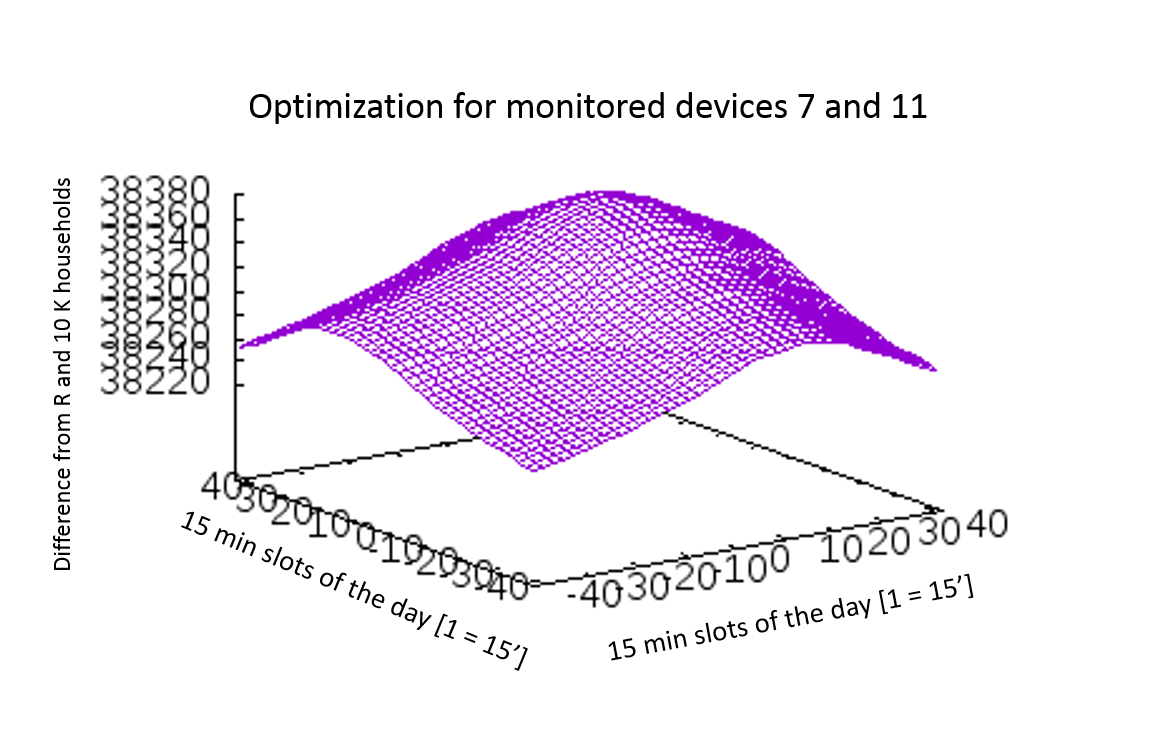
\includegraphics[scale=0.3]{hyper_labels}
  \end{minipage}


}

\frame{\frametitle{And how does this help us?}


\begin{minipage}{.5\textwidth}
\centering
    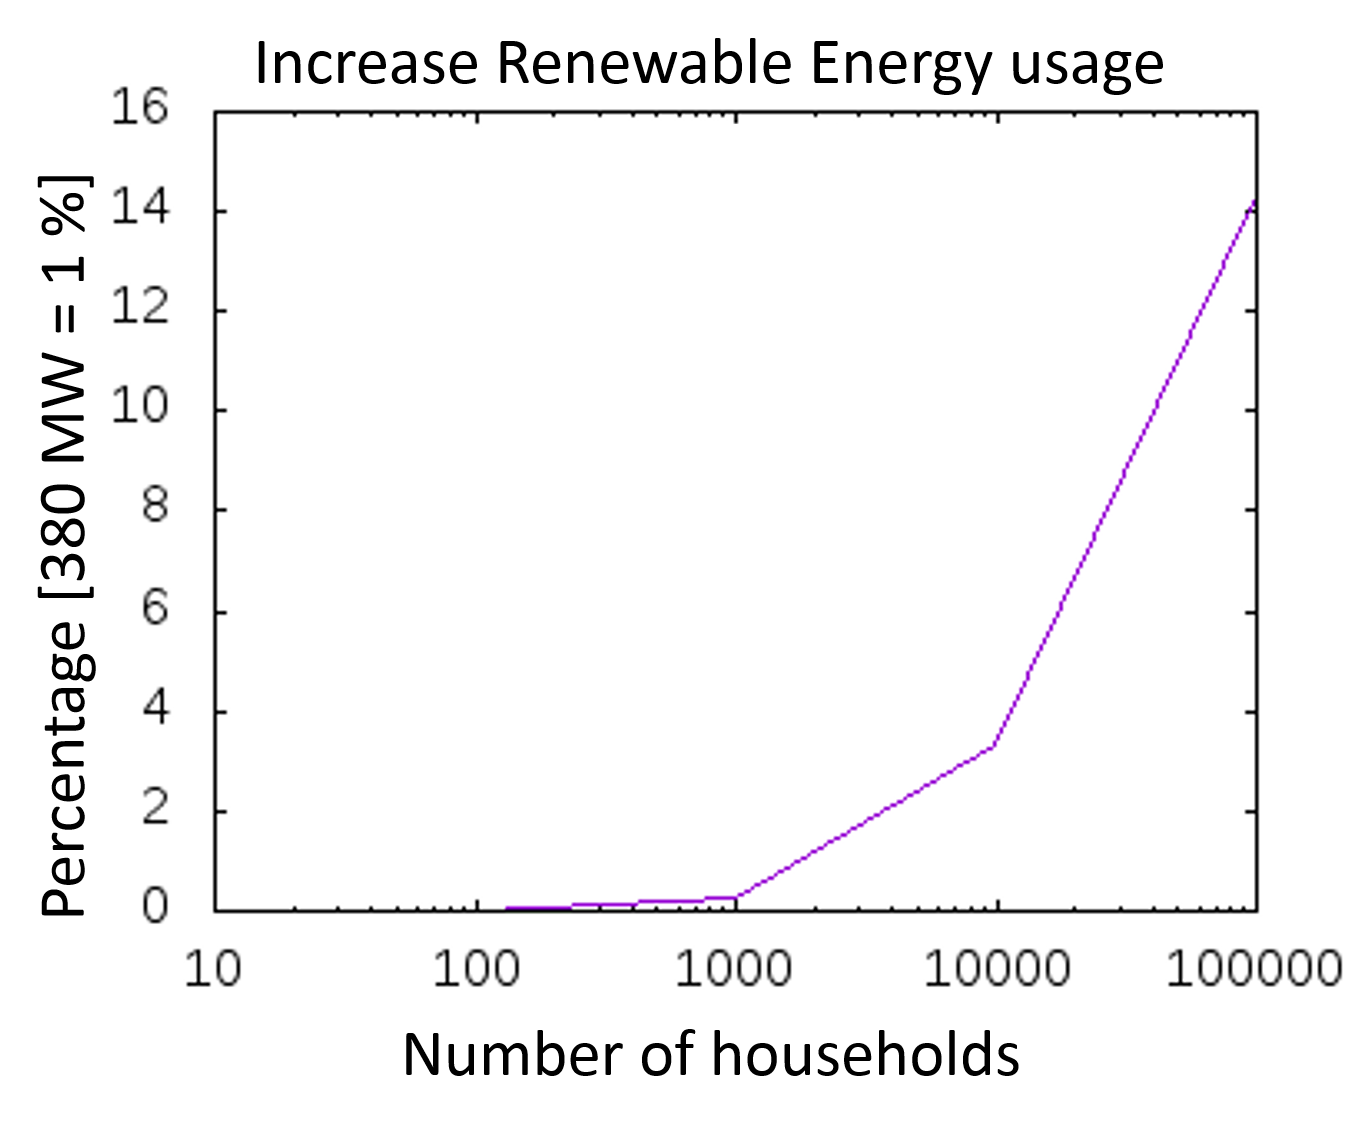
\includegraphics[scale=.2]{pot_labels_perc}
  \end{minipage}%
  \begin{minipage}{.5\textwidth}
    \centering
    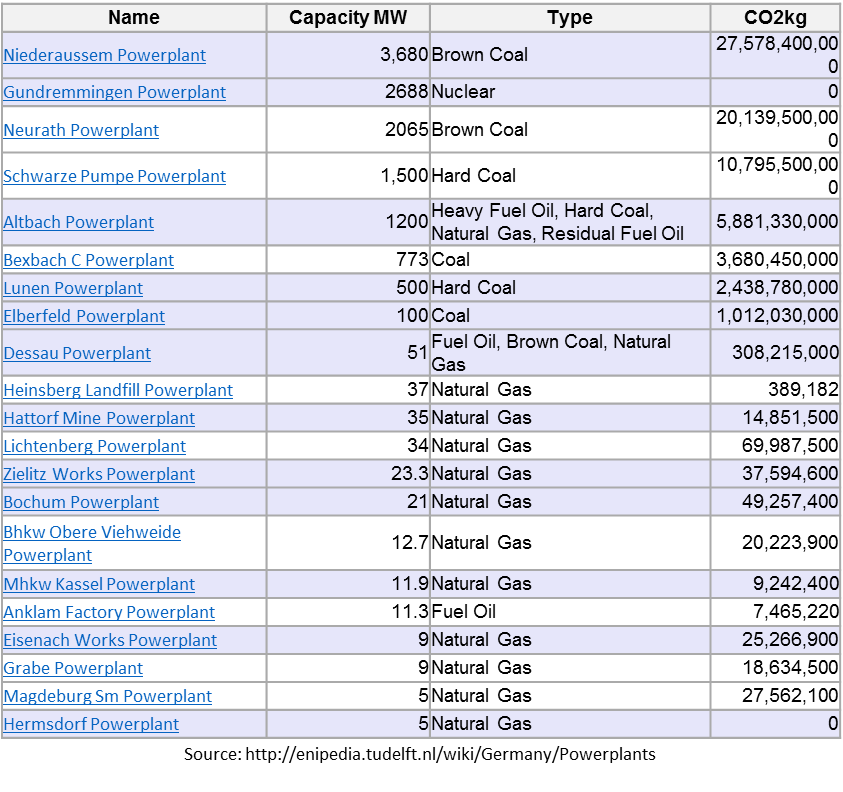
\includegraphics[scale=0.35]{lits_power_plants}
  \end{minipage}

}

\end{document}
